\newpage
 La imagen\autoref{fig:FLECHAS} se puede observar los dos elementos y la fuerza resultante de la desviación generada por la rotación. Las fuerzas F son generadas por la resonancia de las piezas en el sistema, las cuales mientras en una parte generan un movimiento resonante de tipo resorte, en la parte central generan un movimiento oscilatorio a una frecuencia previamente programada. Al momento de estar presente la rotación, se genera una desviación en las fuerzas, señalada en la imagen como S \cite{SICK_Encodersd}. Esto a su vez genera una desviación en las oscilaciones de la parte central de la pieza, lo cual provoca una diferencia en la frecuencia previamente programada, siendo esta diferencia detectada por una zona dentada del mecanismo.

El cambio de frecuencia se consideraría en este caso como cambio de posición en el espacio. 

Este proceso funciona de la misma manera en los tres ejes, dando así la capacidad a los dispositivos de saber en qué posición se encuentran dentro del espacio.
\begin{figure}[h]
	\centering
	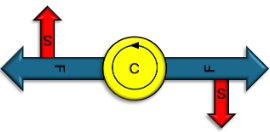
\includegraphics[width=0.3\linewidth]{img/FLECHAS}
	\caption{Direccion de fuerzas  }
	\label{fig:FLECHAS}
\end{figure}

\section{ACELEROMETRO}

Los acelerómetros\autoref{fig:ACE},se utilizan en mediciones de aceleración gravitacional estática como se aprecia en \cite{TME_Acelerometro}, lo que le permite determinar el ángulo de desviación del objeto medido de la vertical, así como en mediciones de aceleración dinámica debido a golpes, movimiento, impacto o vibración, es decir, vibraciones de baja amplitud y baja frecuencia, que alcanzan varias docenas de Hz.
\begin{figure}[h]
	\centering
	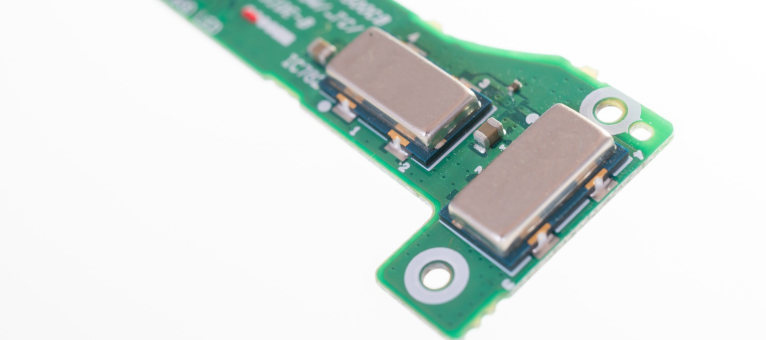
\includegraphics[width=0.3\linewidth]{img/ACE}
	\caption{Acelerometro }
	\label{fig:ACE}
\end{figure}


¿Cómo funciona un acelerómetro mientras se mide la vibración? Este dispositivo se implementa directamente en el objeto que vibra, lo que le permite convertir la energía de vibración en una señal eléctrica que es proporcional a la aceleración momentánea del objeto.

¿Qué hace un acelerómetro? La medición de la vibración se usa generalmente para diagnosticar el funcionamiento de máquinas, dispositivos o estructuras sometidas a altos esfuerzos, por ejemplo, estructuras de acero de mástiles, puentes o estructuras de edificios. También se utilizan acelerómetros, entre otros. para proteger los discos duros contra daños, en equipos médicos y deportivos, en cámaras y videocámaras, en teléfonos inteligentes, controles remotos, controladores o en sistemas de navegación.

¿Qué es un acelerómetro? No es más que un transductor de aceleración que mide su propio movimiento en el espacio. Hay tres tipos básicos de acelerómetros, más de los cuales más adelante en el artículo.

